%%%%%%%%%%%%%%%%%%%%%%%%%%%%%%%%%%%%%%%%%
% Beamer Presentation
% LaTeX Template
% Version 1.0 (10/11/12)
%
% This template has been downloaded from:
% http://www.LaTeXTemplates.com
%
% License:
% CC BY-NC-SA 3.0 (http://creativecommons.org/licenses/by-nc-sa/3.0/)
%
%%%%%%%%%%%%%%%%%%%%%%%%%%%%%%%%%%%%%%%%%

%----------------------------------------------------------------------------------------
%	PACKAGES AND THEMES
%----------------------------------------------------------------------------------------

\documentclass[14pt,handout]{beamer}
%%\documentclass[14pt]{beamer}

\mode<presentation> {

% The Beamer class slide themes
\usetheme{Madrid} %i was using this one

% Beamer class color themes

%\usecolortheme{albatross}

%\setbeamertemplate{footline} % To remove the footer line in all slides uncomment this line
%\setbeamertemplate{footline}[page number] % To replace the footer line in all slides with a simple slide count uncomment this line

%\setbeamertemplate{navigation symbols}{} % To remove the navigation symbols from the bottom of all slides uncomment this line
}

\usepackage{graphicx} % Allows including images
\usepackage{booktabs} % Allows the use of \toprule, \midrule and \bottomrule in tables
\usepackage{hyperref}
\usepackage{helvet}
\usepackage[T1]{fontenc}
\usepackage{textcomp}

%----------------------------------------------------------------------------------------
%	TITLE PAGE
%----------------------------------------------------------------------------------------

\title[RNAseq Practical pt1]{RNAseq Analysis: A Practical Walkthrough (part 1/n)} % The short title appears at the bottom of every slide, the full title is only on the title page

\author{C. Ryan Campbell} % Your name
\institute[Duke] % Your institution as it will appear on the bottom of every slide, may be shorthand to save space
{
Duke University \\ % Your institution for the title page
\medskip
\textit{c.ryan.campbell@duke.edu} % Your email address
}
\date{12 Oct 2017} % Date, can be changed to a custom date

\begin{document}

\begin{frame}
\titlepage % Print the title page as the first slide
\end{frame}

\begin{frame}
\frametitle{Overview} % Table of contents slide, comment this block out to remove it
\tableofcontents % Throughout your presentation, if you choose to use \section{} and \subsection{} commands, these will automatically be printed on this slide as an overview of your presentation
\end{frame}

%----------------------------------------------------------------------------------------
%	PRESENTATION SLIDES
%----------------------------------------------------------------------------------------

%------------------------------------------------
\begin{frame}
\frametitle{Today's Goals}
\begin{itemize}
	\item<+-> Clean Data
	\item<+-> Prepare genome files
	\item<+-> Run tophat2 (?)
	\begin{itemize}
		\item<+-> (at least give you the tools to run it...)
	\end{itemize}
\end{itemize}
\end{frame}

%------------------------------------------------
\section{Workflow}
%------------------------------------------------

%------------------------------------------------
\begin{frame}
\frametitle{Workflow}
\begin{enumerate}
	\large
	\item<+-> Get in your groups
	\item<+-> Fill in the missing blanks on my diagram
	\begin{itemize}
		\item<+-> Fill in a description and software
		\item<+-> Should take about 10 minutes
	\end{itemize}
\end{enumerate}
\end{frame}

%------------------------------------------------
\begin{frame}
\frametitle{slogin OR sbatch script}
\begin{itemize}
	\large
	\item<+-> What is the difference?
	\item<+-> Make sure you're making a conscious choice between the two
	\item<+-> Today we'll be working on slogin with \underline{SMALL} files
	\item<+-> (why does this matter?)
	\item<+-> When you analyze your files, make sure to use an sbatch script
\end{itemize}
\end{frame}

%------------------------------------------------
\section{Data Quality}
%------------------------------------------------

%------------------------------------------------
\begin{frame}
\frametitle{Data Quality}
\begin{itemize}
	\item<+-> So far you've downloaded data
	\item<+-> Next step is to check the quality
	\item<+-> And if the qulity is poor, ``trim'' the data
\end{itemize}
\end{frame}

%------------------------------------------------
\begin{frame}
\frametitle{Data Quality}
\begin{itemize}
	\item<+-> This will simultaneously accomplish two goals:
	\begin{enumerate}
		\large
		\item<+-> Check that the data is as expected (length, format)
		\begin{itemize}
			\item<+-> Important because you otherwise can't see the data
		\end{itemize}
		\item<+-> Confirm that the data is a good quality across samples
	\end{enumerate}
	\item<+-> We'll be using \href{https://www.bioinformatics.babraham.ac.uk/projects/fastqc/}{fastqc}
\end{itemize}
\end{frame}

%------------------------------------------------
\subsection{fastqc}
%------------------------------------------------

%------------------------------------------------
\begin{frame}
\frametitle{fastqc}
\begin{itemize}
	\item Runs on the cluster - (small files on slogin, large as an sbatch)
	\item Output html file describes the fastq file (length, base composition, phred score quality, etc)
	\item To run fastqc:
	\footnotesize
	\ttfamily
	\begin{block}{}
	\item[] cd /work/cc216/490S/<your netid>
	\item[] export PATH=/work/cc216/490S/software/FastQC/:\$PATH
	\item[] EXAMPLE: fastqc [-f fastq|bam|sam] seqfile1 seqfile2 .. seqfileN 
	\item[] fastqc -f fastq /work/cc216/490S/cc216/test\_data/RNAseq\_r1.fq  /work/cc216/490S/cc216/test\_data/RNAseq\_r2.fq
	\end{block}
	\sffamily
	\item The html output is generated but on the cluster, what is the last step?
\end{itemize}
\end{frame}

%------------------------------------------------
\begin{frame}
\frametitle{fastqc output}
\begin{columns}
	\begin{column}{0.35\textwidth}
		\begin{itemize}
			\item \underline{Run Quality}
			\item Base Content
			\item Run Length
		\end{itemize}
		\end{column}
	\begin{column}{0.65\textwidth}
		\begin{center}
     		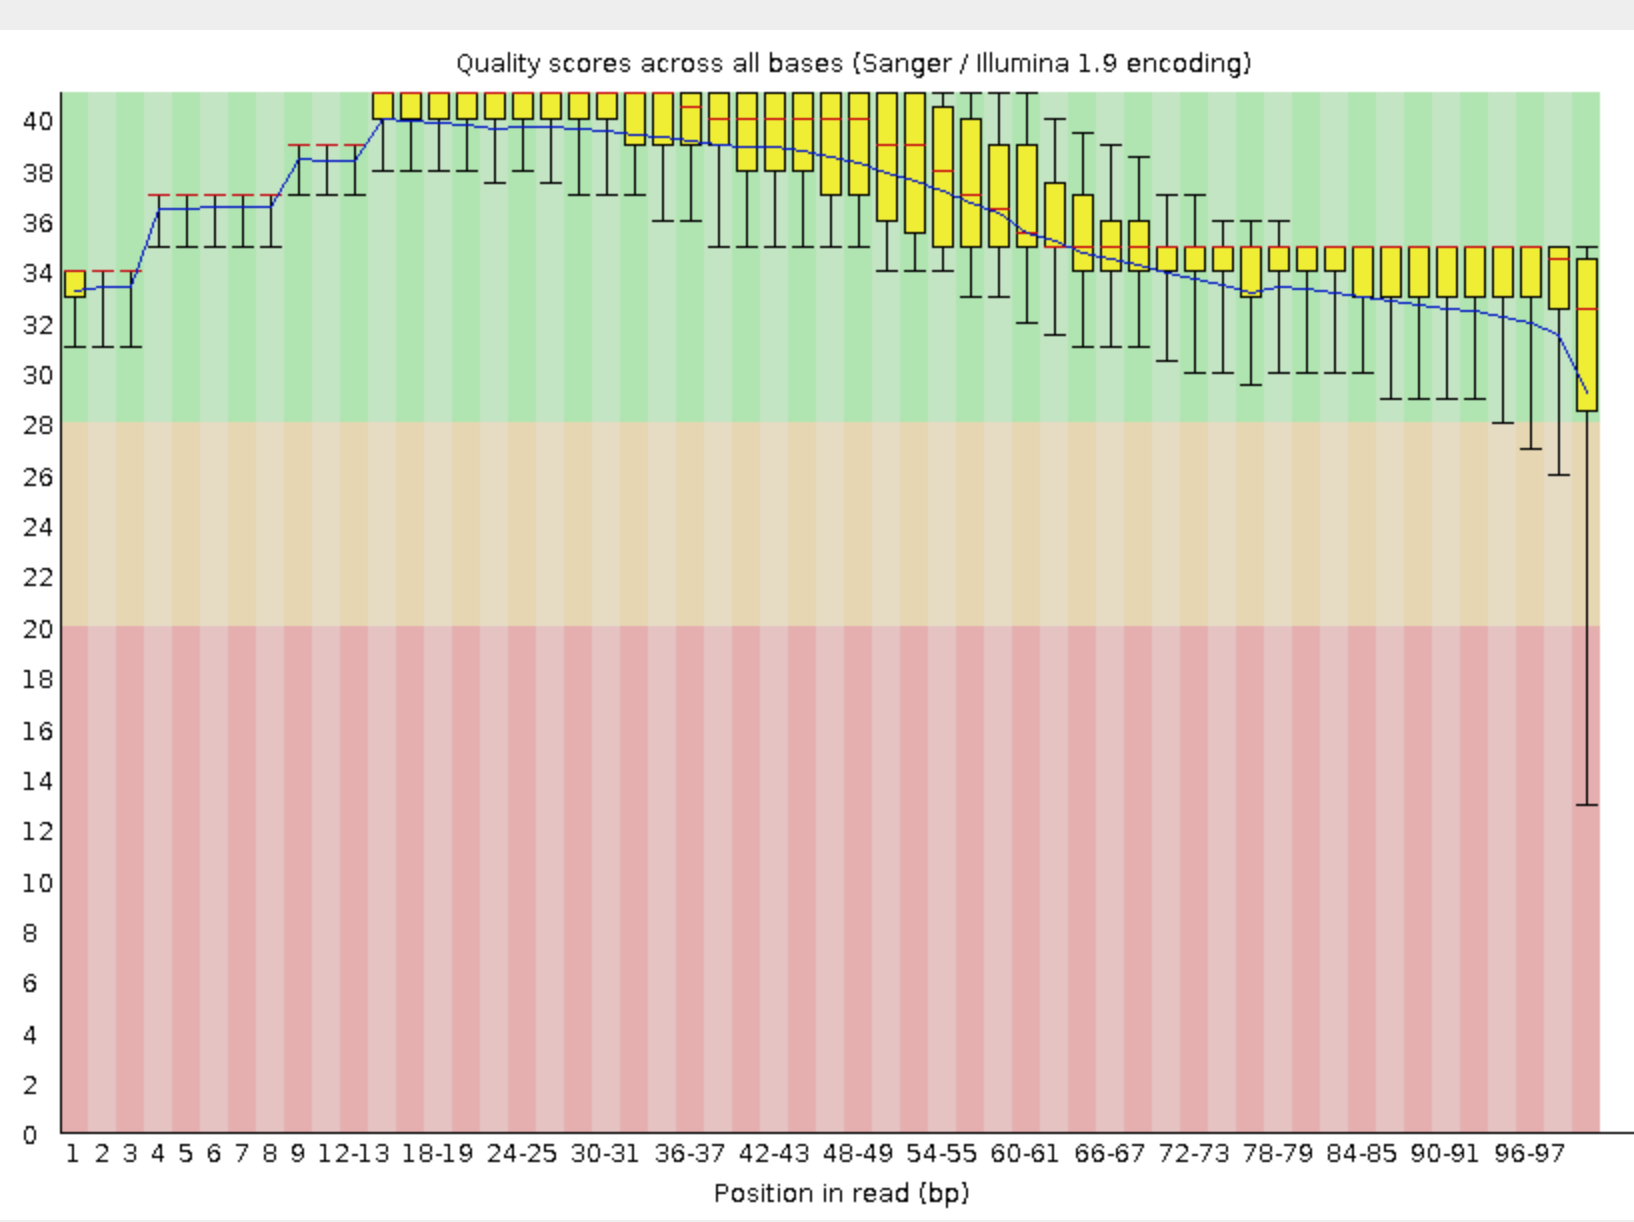
\includegraphics[width=1\textwidth]{/Users/ryan/Documents/git_repos/duke-bio490s/slides/images_20171012_run_qual.png}
     	\end{center}
	\end{column}
\end{columns}
\end{frame}

%------------------------------------------------
\begin{frame}
\frametitle{fastqc output}
\begin{columns}
	\begin{column}{0.35\textwidth}
		\begin{itemize}
			\item Run Quality
			\item \underline{Base Content}
			\item Run Length
		\end{itemize}
		\end{column}
	\begin{column}{0.65\textwidth}
		\begin{center}
     		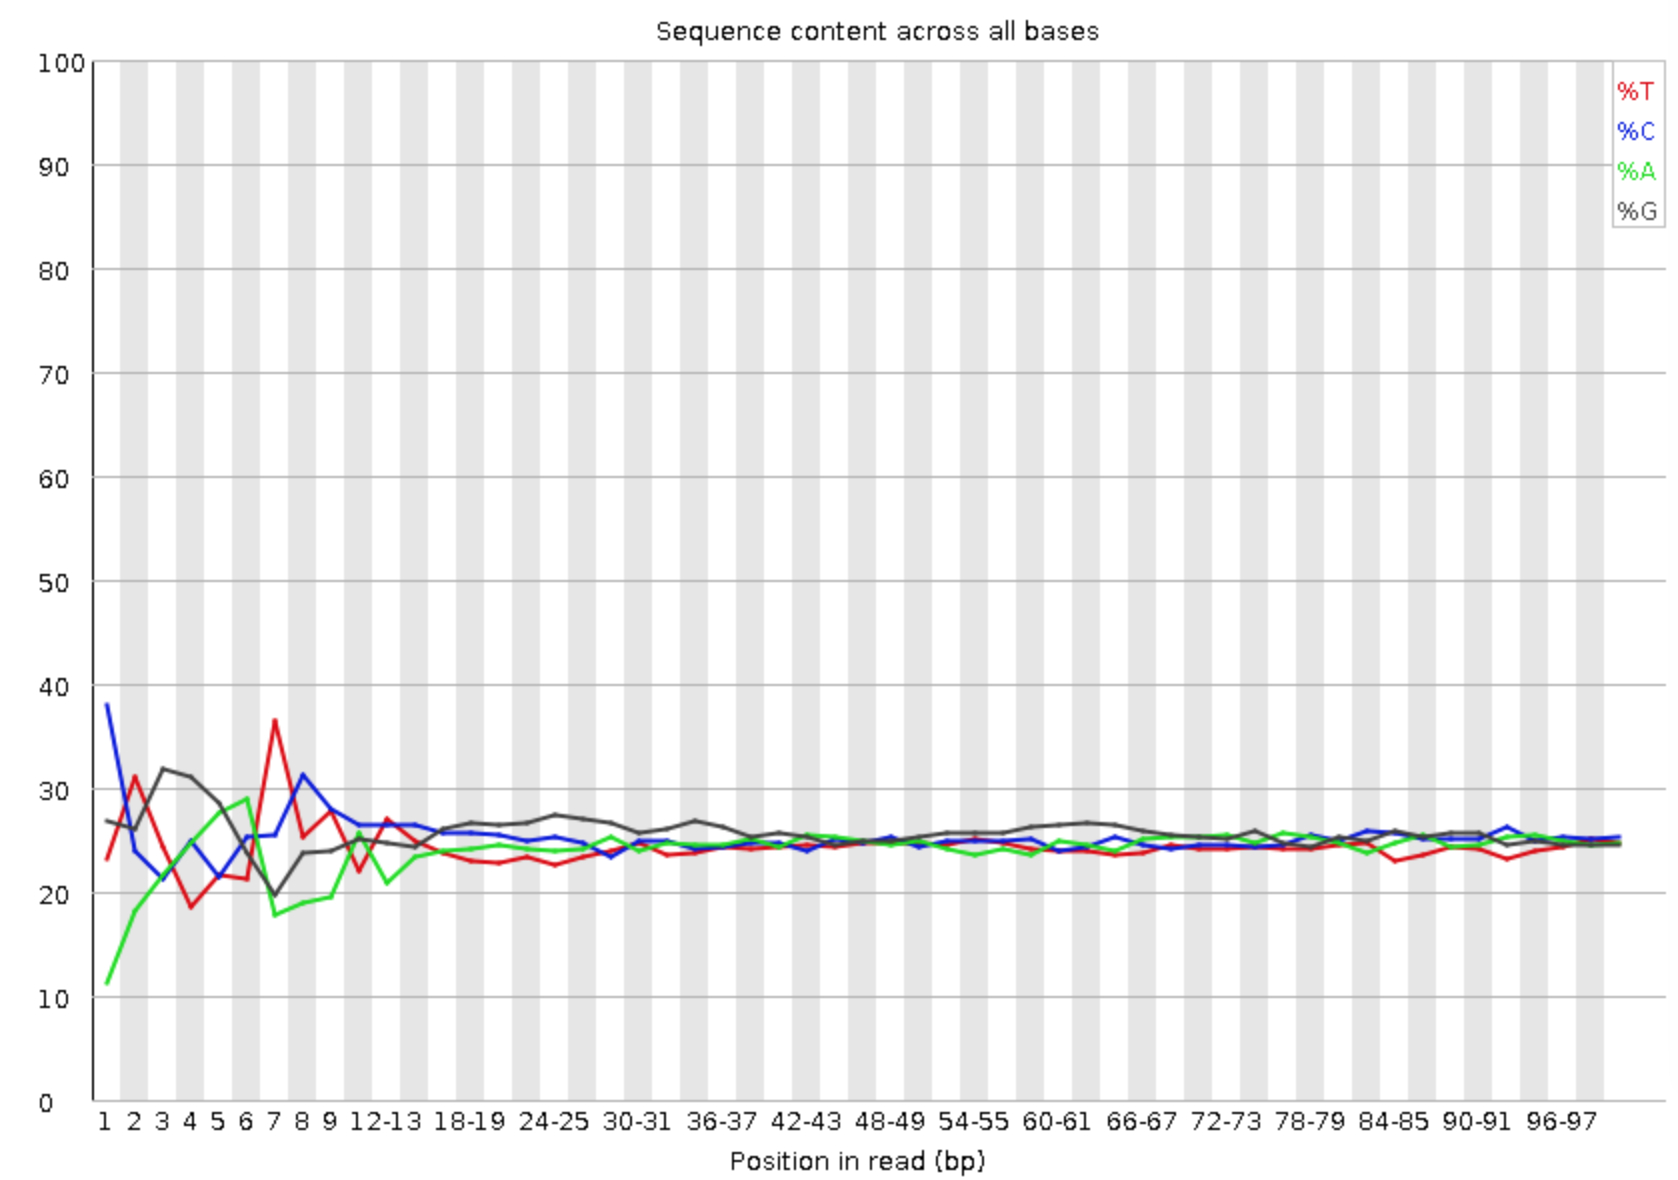
\includegraphics[width=1\textwidth]{/Users/ryan/Documents/git_repos/duke-bio490s/slides/images_20171012_base_content.png}
     	\end{center}
	\end{column}
\end{columns}
\end{frame}

%------------------------------------------------
\begin{frame}
\frametitle{fastqc output}
\begin{columns}
	\begin{column}{0.35\textwidth}
		\begin{itemize}
			\item Run Quality
			\item Base Content
			\item \underline{Run Length}
		\end{itemize}
		\end{column}
	\begin{column}{0.65\textwidth}
		\begin{center}
     		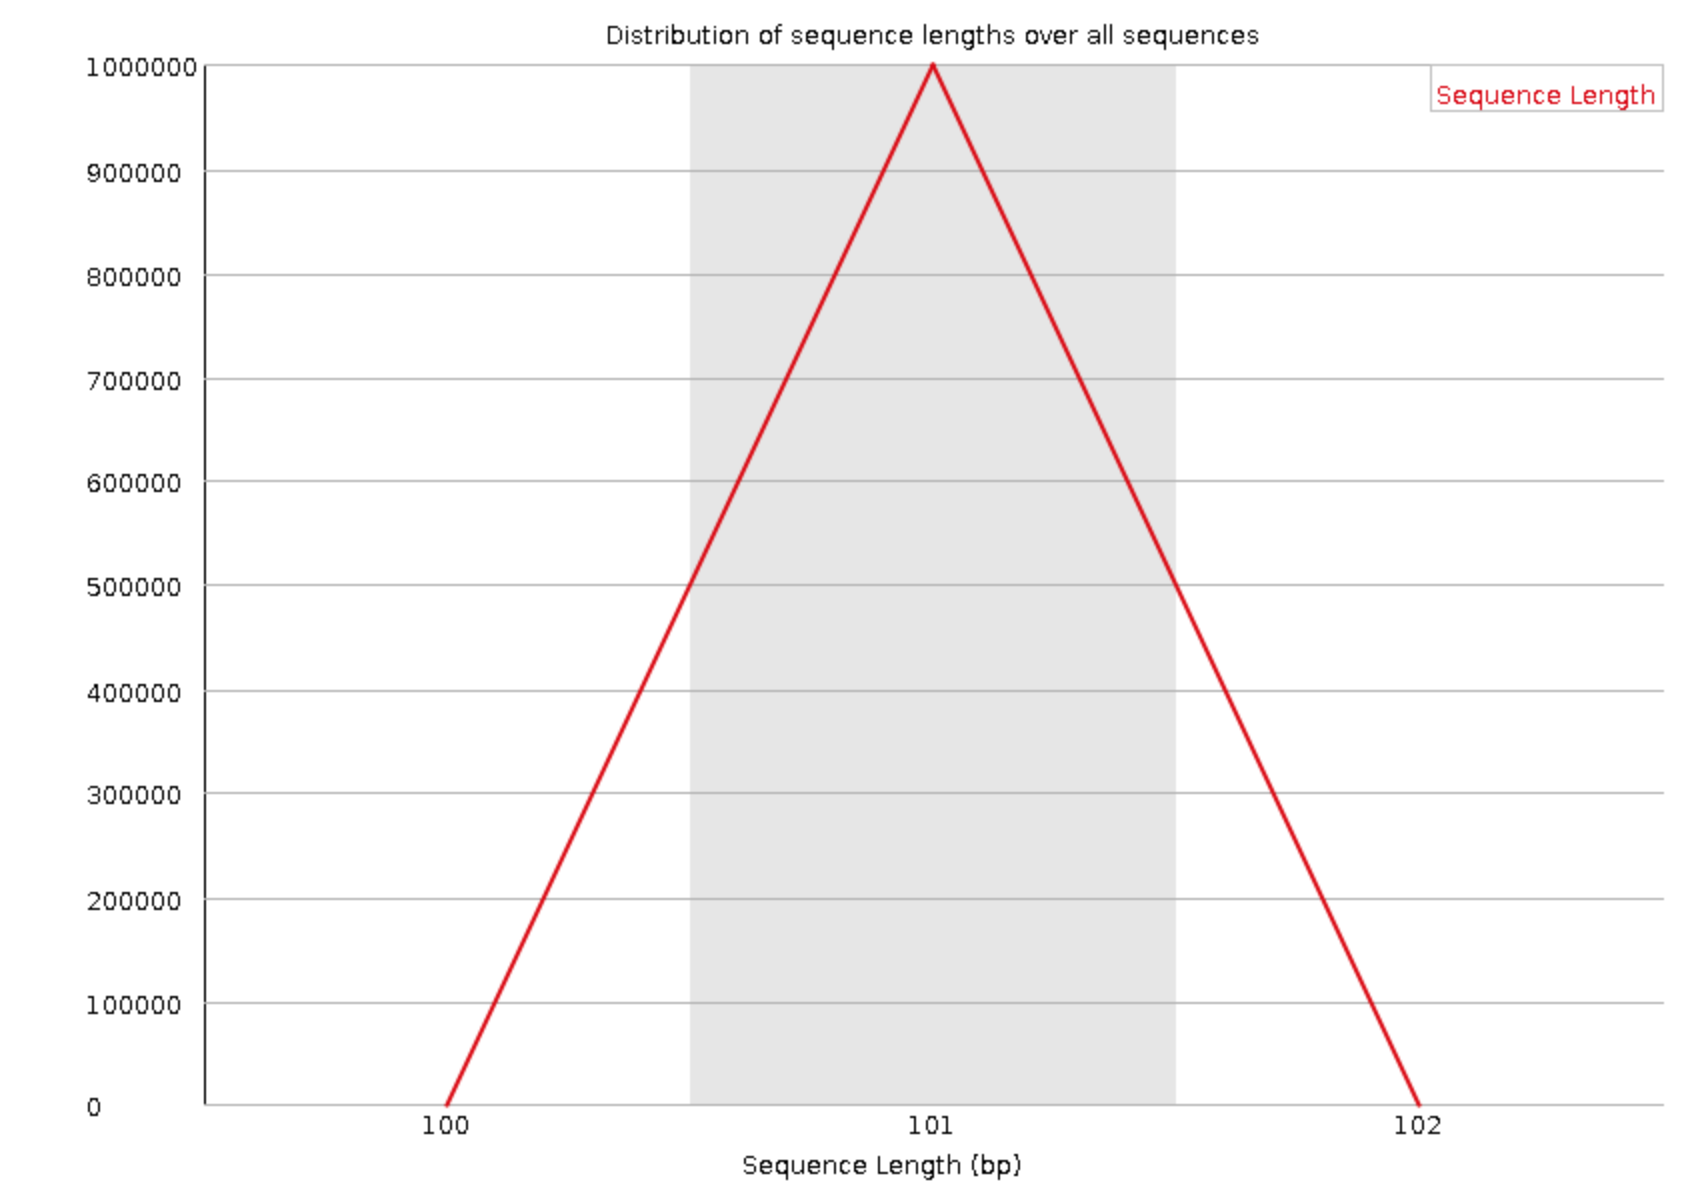
\includegraphics[width=1\textwidth]{/Users/ryan/Documents/git_repos/duke-bio490s/slides/images_20171012_run_length.png}
     	\end{center}
	\end{column}
\end{columns}
\end{frame}

%------------------------------------------------
\subsection{trimmomatic}
%------------------------------------------------

%------------------------------------------------
\begin{frame}
\frametitle{Trimming Data}
\begin{itemize}
	\item<+-> Remove data that is low quality
	\begin{itemize}
		\item<+-> You have \underline{TONS} of data, taking out 5\% is OK
	\end{itemize}
	\item<+-> We will set a couple of parameters:
	\begin{itemize}
		\item<+-> Minimum quality at the end of the read
		\item<+-> Average quality along a sliding window
		\item<+-> Overall read quality
	\end{itemize}
	\item<+-> If the read doesn't meet some, or all, of these the whole read is tossed
	\item<+-> We'll be using \href{http://www.usadellab.org/cms/?page=trimmomatic}{trimmomatic}
\end{itemize}
\end{frame}

%------------------------------------------------
\begin{frame}
\frametitle{trimmomatic}
\begin{itemize}
	\item Runs on the cluster (sbatch script)
	\item Writes a new fastq file (or pair, R1 \& R2)
	\item To run trimmomatic:
	\tiny
	\ttfamily
	\begin{block}{}
	\item[] cd /work/cc216/490S/<your netid>
	\item[] EXAMPLE:
	\item[] java -jar /work/cc216/490S/software/Trimmomatic-0.36/trimmomatic-0.36.jar PE -phred33 -trimlog RNAseq.trimlog RNAseq\_r1.fastq RNAseq\_r2.fastq RNAseq\_r1.trimm.5.20.fastq RNAseq\_r1.trimm.unpaired.5.20.fastq RNAseq\_r2.trimm.5.20.fastq RNAseq\_r2.trimm.unpaired.5.20.fastq LEADING:3 TRAILING:3 SLIDINGWINDOW:5:20 MINLEN:50
	\end{block}
	\sffamily
	\footnotesize
	\item trimmomatic is a java file, you're essentially running the command ``java'' then pointing it to the .jar file for instructions
	\item Do you need to move this file down to your laptop?
\end{itemize}
\end{frame}

%------------------------------------------------
\begin{frame}
\frametitle{trimmomatic example}
\begin{itemize}
	\item To run trimmomatic:
	\ttfamily
	\footnotesize
	\begin{block}{}
	\item[] EXAMPLE:
	\item[] java -jar /work/cc216/490S/software/Trimmomatic-0.36/trimmomatic-0.36.jar <PE or SE> -phred33 -trimlog <output log> <Read 1.fq> <Read 2.fq> <Read 1 output> <Read 1 output unpaired> <Read 2 output> <Read 2 output unpaired> LEADING:3 TRAILING:3 SLIDINGWINDOW:5:20 MINLEN:50
	\end{block}
	\sffamily
	\item Remove (leading/trailing) low quality or N bases (below quality 3)
	\item Scan the read with a 5-base wide sliding window, cutting when the average quality per base drops below 20
	\item Drop reads which are less than 50 bases long after these steps
\end{itemize}
\end{frame}

%------------------------------------------------
\begin{frame}
\frametitle{trimmomatic example}
\begin{itemize}
	\item Output:
	\ttfamily
	\footnotesize
	\begin{block}{}
	\item[] Input Read Pairs: 1000000 Both Surviving: 955447 (95.54\%) Forward Only Surviving: 29029 (2.90\%) Reverse Only Surviving: 9577 (0.96\%) Dropped: 5947 (0.59\%)
	\item[] >head RNAseq.log
	\item[] SRR848963.63 ILLUMINA:322:D0UFKACXX:3:1101:11445:2184 length=101 101 0 101 0
	\item[] SRR848963.64 ILLUMINA:322:D0UFKACXX:3:1101:11909:2032 length=101 97 1 98 3
	\item[] SRR848963.64 ILLUMINA:322:D0UFKACXX:3:1101:11909:2032 length=101 98 0 98 3
	\end{block}
\end{itemize}
\end{frame}

%------------------------------------------------
\begin{frame}
\frametitle{trimmomatic}
\begin{itemize}
	\item<+-> At this point, you should run fastqc again
	\item<+-> Why?
	\item<+-> Check that trimmomatic improved the quality
	\item<+-> Check that trimmomatic fixed specific problems
	\item<+-> Always want to assess your final product
\end{itemize}
\end{frame}

%------------------------------------------------
\section{Genomes}
%------------------------------------------------

%------------------------------------------------
\begin{frame}
\frametitle{So you say you need a genome...}
\begin{itemize}
	\large
	\item<+-> Why do we need a genome?
	\item<+-> Where do we get it?
	\item<+-> And if you don't know...
\end{itemize}
\end{frame}

%------------------------------------------------
\subsection{Downloading}
%------------------------------------------------

%------------------------------------------------
\begin{frame}
\frametitle{Downloading genomes}
\begin{columns}
	\begin{column}{0.3\textwidth}
		\begin{itemize}
			\footnotesize
			\item<+-> Hopefully your googling led you to NCBI
			\item<+-> Model species have a page like this
			\item<+-> Download from the ``FASTA format for genome'' and ``annotation in GFF'' links
		\end{itemize}
		\end{column}
	\begin{column}{0.7\textwidth}
		\begin{center}
     		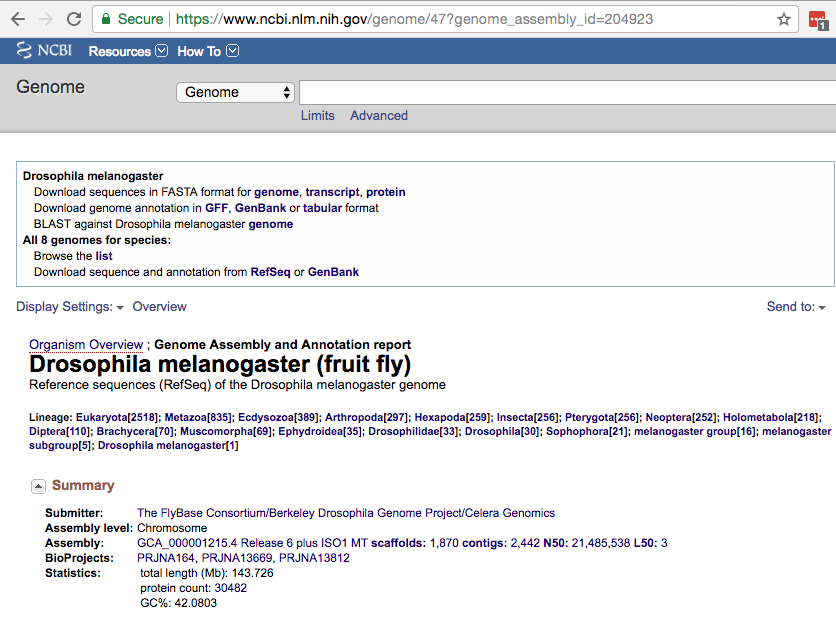
\includegraphics[width=1\textwidth]{/Users/ryan/Documents/git_repos/duke-bio490s/slides/images_20171012_fly_genome.png}
     	\end{center}
	\end{column}
\end{columns}
\end{frame}

%------------------------------------------------
\subsection{Indexing}
%------------------------------------------------

%------------------------------------------------
\begin{frame}
\frametitle{Indexing}
\begin{itemize}
	\large
	\item<+-> Most aligners require their genome to be indexed
	\item<+-> What do you think this means?
	\item<+-> You'll need to index using bowtie2 (the aligner tophat2 uses)
\end{itemize}
\end{frame}

%------------------------------------------------
\begin{frame}
\frametitle{Indexing}
\begin{itemize}
	\large
	\item<+-> Most aligners require their genome to be indexed
	\item<+-> What do you think this means?
	\item<+-> You'll need to index using bowtie2 (the aligner tophat2 uses)
\end{itemize}
\end{frame}

%------------------------------------------------
\begin{frame}
\frametitle{bowtie index}
\begin{itemize}
	\item This is going to be a computationally intensive process
	\item So write a submission script to do it
	\item You can start with my template:
	\footnotesize
	\ttfamily
	\begin{block}{}
	\item[] export PATH=/opt/apps/tophat-bowtie/:\$PATH
	\item[]
	\item[] cat /work/cc216/490S/cc216/genome\_index.submit
	\item[] cp /work/cc216/490S/cc216/genome\_index.submit /work/cc216/490S/duke-bio490s/projects/<your\_project>/
	\end{block}
	\sffamily
	\item Now, edit the file to index the genome you downloaded, in your folder
\end{itemize}
\end{frame}

%------------------------------------------------
\section{Data Prep}
%------------------------------------------------

%------------------------------------------------
\begin{frame}
\frametitle{Preparing your data files}
\begin{itemize}
	\item<+-> We're now ready to align the RNAseq reads to the genome
	\item<+-> At this point, you're going to start generating a lot of different files
	\item<+-> So this is a good point to plan out file names with your group
	\item<+-> So that everyone knows which files are which, it is best to rename files:
	\begin{itemize}
		\footnotesize
		\item<+-> e.g. change SRR1201401\_1.fastq to adultSample1\_r1.fastq
		\item<+-> Keep a file with a record of these changes
		\item<+-> (The same file can be a for loop to make the changes)
	\end{itemize}
\end{itemize}
\end{frame}

%------------------------------------------------
\section{Alignment}
%------------------------------------------------

%------------------------------------------------
\subsection{tophat}
%------------------------------------------------

%------------------------------------------------
\begin{frame}
\frametitle{tophat}
\begin{itemize}
	\item tophat2 is the command/software that aligns the reads to the genome
	\item This (also) is going to be a computationally intensive process
	\item So write a submission script to do it:
	\footnotesize
	\ttfamily
	\begin{block}{}
	\item[] export PATH=/opt/apps/tophat-bowtie/:\$PATH
	\item[]
	\item[] tophat2
	\end{block}
	\sffamily
	\item No template this time!
	\item Run tophat2 command and read over the manual
	\item The next slide has an example command -- be careful, the defaults are suitable for mammals, if you're working with non-mammalian data check your paper to for suggestions
\end{itemize}
\end{frame}

%------------------------------------------------
\begin{frame}
\frametitle{tophat}
\begin{itemize}
	\item tophat2 example (all one line):
	\footnotesize
	\ttfamily
	\begin{block}{}
	\item[]  tophat -p 4 -o RNAseq1 -G /work/cc216/490S/cc216/genomes/dmel\_20171011.gff dmel /work/cc216/490S/cc216/test\_data/RNAseq\_r1.trimm.5.20.fastq /work/cc216/490S/cc216/test\_data/RNAseq\_r2.trimm.5.20.fastq
	\item[] 
	\end{block}
	\sffamily
	\item[] translated:
	\ttfamily
	\begin{block}{}
	\item[]  tophat -p <number of threads> -o <output dir> -G <gff file, annotations> <bowtie2 index> <R1 fastq> <R2 fastq>
	\item[] 
	\end{block}
	\sffamily
	\item Help can be found by running ``tophat2''
	\item On in the tophat2 manual online
	\item \href{http://ccb.jhu.edu/software/tophat/manual.shtml}{http://ccb.jhu.edu/software/tophat/manual.shtml}
\end{itemize}
\end{frame}


%------------------------------------------------
\begin{frame}
\Huge{\centerline{The End}}
\end{frame}

%----------------------------------------------------------------------------------------

\end{document} 